\section{Lenia} \label{sec:lenia}

\subsection{Conway's Game of Life}
Conway's Game of Life ist ein von John Conway entwickeltes Spiel, das auf einem zweidimensionalen Gitter basiert und einen Mikrokosmos simuliert.
Es verwendet einen zweidimensionalen, zellulären Automaten, bei dem die Zellen zu Beginn entweder lebendig oder tot sein können.
Der Folgezustand jeder Zelle wird durch die Anzahl der lebendigen Nachbarzellen in der Moore-Nachbarschaft bestimmt.
Eine lebendige Zelle bleibt im nächsten Schritt lebendig, wenn sie zwei oder drei lebendige Nachbarn hat.
Eine tote Zelle wird im nächsten Schritt lebendig, wenn sie genau drei lebendige Nachbarn hat.
In allen anderen Fällen wird die Zelle im nächsten Schritt tot sein.
Dies führt zu einem geschlossenen System, das sich selbständig weiterentwickelt \cite{wikipedia_gol}.


\begin{figure}[!htbp]\centering
    \begin{subfigure}[t]{0.2\textwidth}
        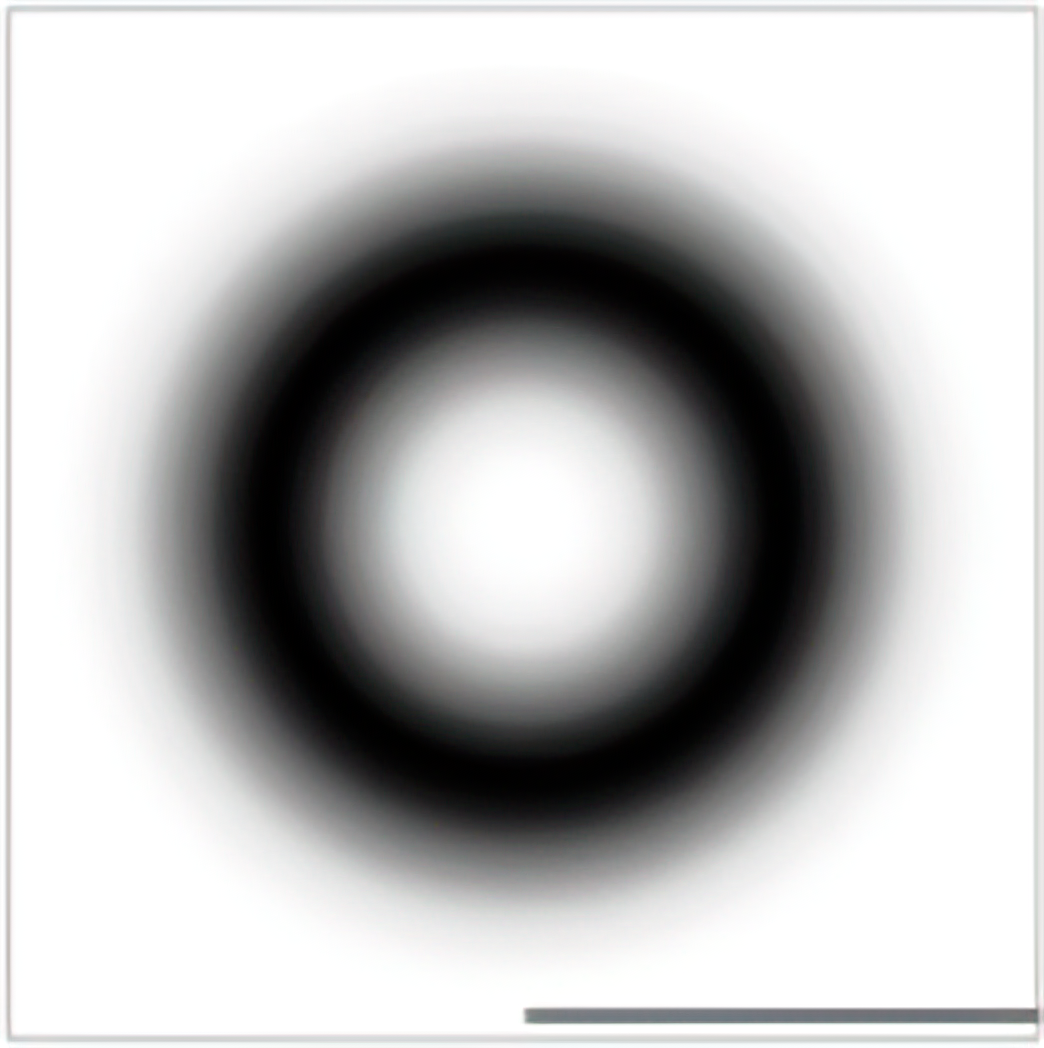
\includegraphics[width=\textwidth]{kernel_shell.png}
        \caption{Kernel-Shell}
        \label{fig:kernels:shell}
    \end{subfigure}
    \hfill
    \begin{subfigure}[t]{0.2\textwidth}
        \centering
        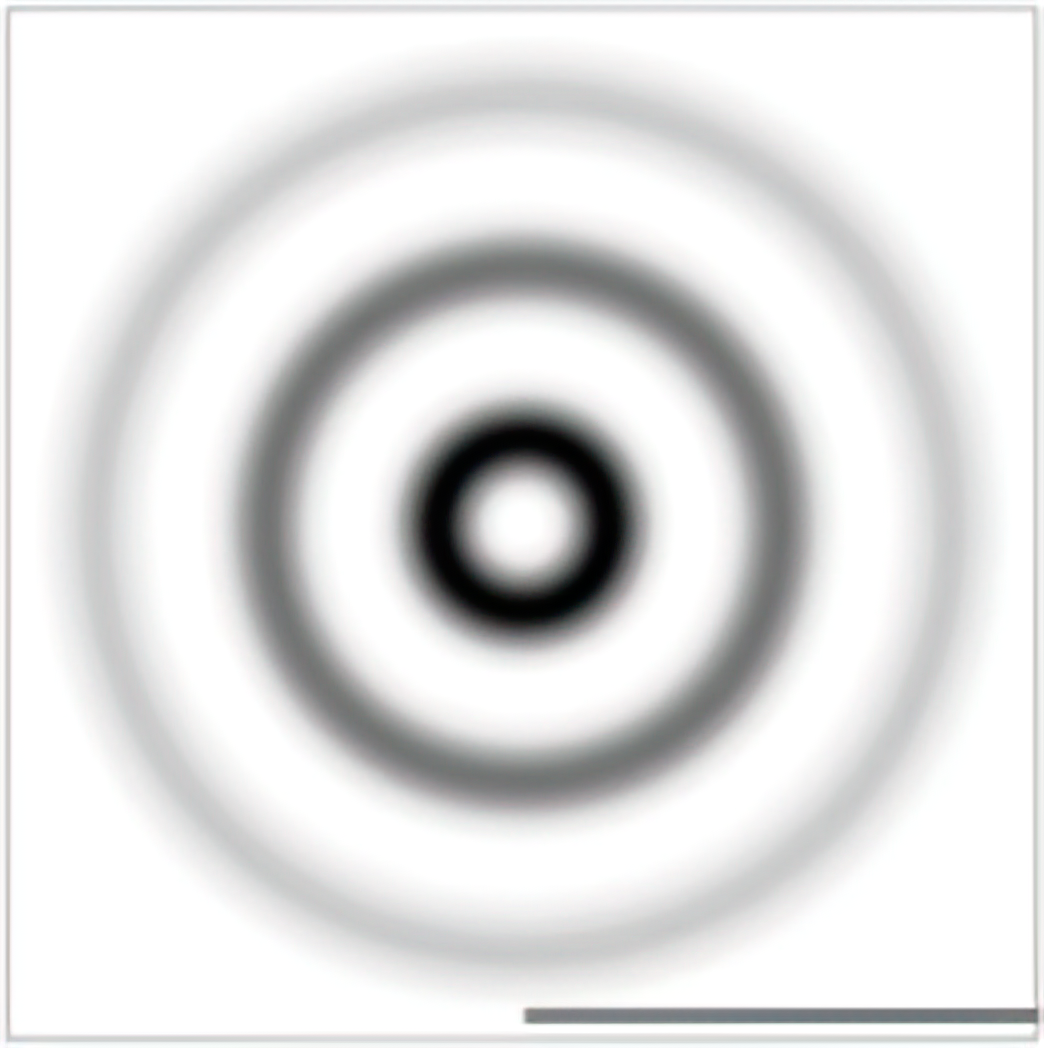
\includegraphics[width=\textwidth]{kernel_skeleton.png}
        \caption{Kernel-Skeleton}
        \label{fig:kernels:skeleton}
    \end{subfigure}
    \caption{\cite{chan2018lenia}}
    \label{fig:kernels}
\end{figure}

\subsection{Lenia}
Der Lenia-Algorithmus gehört ebenfalls zur Familie der zellulären Automaten, unterscheidet sich jedoch von Conway's Game of Life durch sein kontinuierliches System.
Eine Zelle kann nicht nur lebendig oder tot sein, sondern auch einen beliebigen Zustand zwischen 0 und 1 annehmen.
Die Moore-Nachbarschaft wurde durch eine von der Distanz abhängige Nachbarschaft ersetzt, die es ermöglicht, die Nachbarschaft zu erweitern und zu gewichten.
Die Regeln von Conway's Game of Life wurden durch eine Kernel- und eine Growth-Funktion ersetzt, die die Veränderung der Zellen im nächsten Schritt bestimmen.
Zuerst wird mithilfe eines Radius eine Nachbarschaft um die Zelle gebildet.
Die Zustände der Zellen in der Nachbarschaft werden dann mit der Kernel-Funktion gewichtet und anschließend mit der Growth-Funktion zu einem neuen Wert zusammengefasst.
Dieser wird gewichtet auf die Zelle addiert und ergibt den neuen Zustand der Zelle.
Der Kernel besteht aus zwei Teilen: der \textit{Kernel-Shell} und dem \textit{Kernel-Skeleton}.
Für die Kernel-Shell kann beispielsweise die Exponentialfunktion $K_C(r) = \exp\left(\operatorname{4 - \frac{4}{4r(1-r)}}\right)$ gewählt werden, welche wie ~\autoref{fig:kernels:shell} aussieht und die Nachbarschaft gewichtet.
Hierbei ist zu beachten, dass der Radius $r$ auf einem Bereich zwischen 0 und 1 normiert ist.
Soll dies nun auf einem Mesh stattfinden, so bietet es sich an, zuerst die durchschnittliche Kantenlänge der Faces zu bestimmen und ein Vielfaches davon als Norm für den Radius zu wählen.
Des Weiteren lässt sich die Distanz zwischen zwei Faces eines Meshes entweder durch die euklidische Distanz oder durch die Distanz auf der Oberfläche bestimmen.
Die geodätische Distanz ist die kürzeste Distanz zwischen zwei Punkten auf einer Oberfläche.
Es gibt verschiedene Algorithmen zur Bestimmung dieser Distanz, die sich in Genauigkeit und Laufzeit unterscheiden.
Die meisten davon sind jedoch darauf ausgelegt, die Distanz zwischen zwei Vertices und nicht zwischen zwei Faces zu bestimmen.
Wird nun zuerst das duale Mesh bestimmt, so wird das Zentrum eines Faces zu einem Vertex und die Kanten zu Faces.
Die Distanz zwischen zwei Faces ist dann die Distanz zwischen den zugehörigen Vertices.
Alle Faces, die innerhalb des Radius liegen, werden dann in die Nachbarschaft aufgenommen.
Zusätzlich zur Kernel-Shell können noch Peaks hinzugefügt werden, welche in das Kernel-Skeleton einfließen.
Die Peaks sind dabei in einer Liste gespeichert $\beta = \{\beta_0, ..., \beta_{n-1}\} \in [0,1]^n$ und das Kernel-Skeleton ergibt sich wie folgt:
\[
    \operatorname{K_S}(r) = \beta_{\lfloor n \cdot r \rfloor} \cdot \operatorname{K_C}(n \cdot r \bmod 1)
\]
$n$ gibt dabei die Anzahl der Peaks an, $r$ ist die zwischen 0 und 1 normierte Distanz und $\bmod 1$ gibt den Nachkommateil von $n \cdot r$ an.
Die für $\beta$ verwendeten Werte geben dabei die Gewichtung der Peaks an. ~\autoref{fig:kernels:skeleton} zeigt ein Beispiel für ein Kernel-Skeleton mit drei verschiedenen Peaks.
Damit der Kernel vollständig ist, muss dieser nun noch normiert werden. Dies geschieht für eine Zelle wie folgt:
\[
    \begin{aligned}
        N                      & := \text{Menge aller Nachbarn der betrachteten Zelle}                                                                                                     \\
        n                      & := \text{ein Nachbar der betrachteten Zelle}                                                                                                              \\
        \operatorname{dist}(n) & := \text {Distanz zwischen betrachteter Zelle und Zelle n}                                                                                                \\
        \operatorname{area}(n) & := \text {Fläche von Zelle n}                                                                                                                             \\
        \operatorname{K}(n)    & := \frac{\operatorname{K_S}(\operatorname{dist}(n))}{\sum_{n \in N} \left(\operatorname{K_S}(\operatorname{dist}(n)) \cdot \operatorname{area}(n)\right)}
    \end{aligned}
\]
Der Nenner sorgt dabei für die Normierung des Kernels, was durch die noch folgenden Gleichungen deutlich wird.
Ist nun der Kernel vollständig, so lässt sich ein Zwischenwert für die Zelle in Abhängigkeit von der Nachbarschaft bestimmen:
\[
    \begin{aligned}
        x                     & := \text{betrachtete Zelle}                                                                                \\
        \operatorname{A}^t(x) & := \text{aktueller Zustand der Zelle x}                                                                    \\
        \operatorname{U}(x)   & = \sum_{n \in N} \left(\operatorname{K}(n) \cdot \operatorname{A}^t(n) \cdot \operatorname{area}(n)\right)
    \end{aligned}
\]
Nachdem der Zwischenwert für die Zelle bestimmt wurde, wird dieser durch die Growth-Funktion zu einem neuen Wert zusammengefasst.
Die Growth-Funktion ist eine beliebige, kontinuierliche Funktion, die den Zwischenwert, welcher zwischen 0 und 1 liegt, auf einen neuen Wert zwischen -1 und 1 abbildet.
Hier kann beispielsweise eine Exponentialfunktion $\operatorname{G}(u) = 2 \cdot \exp \left(-\frac{(u - \mu)^2}{2 \cdot \sigma^2}\right) - 1$ gewählt werden.
Die Parameter $\mu$ und $\sigma$ können dabei frei angepasst werden.
$\mu$ gibt das Maximum und $\sigma$ die Breite der Funktion an.
~\autoref{fig:expgrowth} zeigt ein Beispiel für verschiedene Parameter.
Ist $\sigma$ ein kleiner Wert, so werden mehr Werte auf -1 abgebildet, wodurch die Zellen schneller sterben.
Nachdem die Growth-Funktion bestimmt wurde, folgt die Aktualisierung der Zelle.
Dafür wird der neue Wert der Zelle mit einem Gewicht auf den alten Wert addiert und zwischen 0 und 1 begrenzt.
\[
    \begin{aligned}
        \operatorname{A}^{t+1}(x)  & := \text{neuer Zustand der Zelle x}                                                                                           \\
        g                          & := \text{Gewichtungsfaktor}                                                                                                   \\
        \operatorname{clip}(u,v,w) & := \operatorname{max}(u, \operatorname{min}(v, w))                                                                            \\
        \operatorname{A}^{t+1}(x)  & := \operatorname{clip}\left(\operatorname{A}^{t+1}(x) + g \cdot \operatorname{G}\left(\operatorname{U}(x)\right), 0, 1\right)
    \end{aligned}
\]
Damit ist die Aktualisierung einer Zelle für einen Zeitschritt abgeschlossen.
Der Gewichtungsfaktor $g \in (0,1]$ und der Zeitschritt $t+1$ bestimmen dabei die zeitliche Auflösung des Systems.
Je kleiner der Gewichtungsfaktor, desto langsamer und flüssiger entwickelt sich das System.

\begin{figure}[!htbp]\centering
    \begin{subfigure}[t]{0.2\textwidth}
        \centering
        \begin{tikzpicture}
            \begin{axis}[
                    axis lines=middle,
                    xmin=0, xmax=1,
                    ymin=-1, ymax=1,
                    xlabel=$u$,
                    ylabel=$\operatorname{G}(u)$,
                    ylabel style={anchor=west},
                    xtick={0,1},
                    ytick={-1,0,1},
                    xticklabels={0,1},
                    yticklabels={-1,0,1},
                    samples=300,
                    width=\textwidth,
                    height=\textwidth,
                ]
                \addplot[domain=-1:1, color=red]{2 * exp(-((x - 0.6)^2)/(2 * 0.1^2)) - 1};
            \end{axis}
        \end{tikzpicture}
        \caption{$\mu = 0.6, \sigma = 0.1$}
        \label{fig:expgrowth:1}
    \end{subfigure}
    \hfill
    \begin{subfigure}[t]{0.2\textwidth}
        \centering
        \begin{tikzpicture}
            \begin{axis}[
                    axis lines=middle,
                    xmin=0, xmax=1,
                    ymin=-1, ymax=1,
                    xlabel=$u$,
                    ylabel=$\operatorname{G}(u)$,
                    ylabel style={at={(1,1)},anchor=east},
                    xtick={0,1},
                    ytick={-1,0,1},
                    xticklabels={0,1},
                    yticklabels={-1,0,1},
                    samples=500,
                    width=\textwidth,
                    height=\textwidth,
                ]
                \addplot[domain=-1:1, color=red]{2 * exp(-((x - 0.15)^2)/(2 * 0.017^2)) - 1};
            \end{axis}
        \end{tikzpicture}
        \caption{$\mu = 0.15, \sigma = 0.017$}
        \label{fig:expgrowth:2}
    \end{subfigure}
    \hfill
    \caption{Exponentialfunktion als Growth-Funktion mit verschiedenen Parametern}
    \label{fig:expgrowth}
\end{figure}

\subsection{Implementierung von Lenia}
Ausgehend davon, dass der Lenia-Algorithmus auf einem statischen Mesh ausgeführt wird, können einige Dinge vorberechnet werden.
Eine naive Implementierung würde für jeden Zeitschritt jede Zelle durchgehen, die Nachbarschaft bestimmen und die benötigten Werte berechnen.
Wenn sich das Mesh und die für den Algorithmus verwendeten Parameter nicht ändern, kann die Nachbarschaft für jede Zelle einmal beim Laden des Meshes bestimmt und danach wiederverwendet werden.
Ebenfalls fällt auf, dass der Wert des Kernels $\operatorname{K}(n)$ von der Distanz zwischen der betrachteten Zelle und der Zelle $n$ abhängt.
Wenn sich die Nachbarschaft einer Zelle nicht ändert, kann der Wert des Kernels für alle Nachbarn einer Zelle einmal berechnet und anschließend wiederverwendet werden.
Hierbei ist zu beachten, dass eine Zelle nicht nur einen Kernel-Wert hat.
Der Kernel-Wert hängt von der Nachbarschaftsrelation ab, weshalb es sinnvoll ist, ihn mit der zuvor erwähnten Nachbarschaftsrelation zu speichern.
Darüber hinaus bleibt die Fläche $\operatorname{area}(n)$ einer Zelle auf einem statischen Mesh konstant, so dass sie ebenfalls vorberechnet werden kann.
Die Kernel-Funktion $\operatorname{K_S}$ und die Funktion $\operatorname{U}$ enthalten beide eine Summe mit derselben Laufvariable und demselben Endwert, sodass sie in der Implementierung in einer Schleife zusammengefasst werden können.
Wenn all diese Werte vorberechnet werden, muss bei der Aktualisierung des Zustands einer Zelle nur der aktuelle Zustand abgefragt und mit bereits berechneten Werten multipliziert werden, um den Kernel-Wert zu erhalten.
Dieser wird dann in die Growth-Funktion eingesetzt und der neue Zustand der Zelle bestimmt.
Bei der Aktualisierung des Zustands des gesamten Systems wird jede Zelle durchlaufen und anhand der zuvor bestimmten Nachbarschaft der neue Zustand bestimmt.
Da der nächste Zustand immer nur vom aktuellen Zustand abhängt, kann dieser Prozess parallelisiert werden.
Der Wert jeder Zelle kann unabhängig von den anderen Zellen bestimmt werden.
Dadurch lässt sich die Berechnung des nächsten Zustands auf mehrere Threads aufteilen und beschleunigen.